\chapter{Systematic Error Analysis}
\minitoc
\label{Cap:ErrorAnalysis}

The MINER$\nu$A experiment implements the \textit{Many-Universes Uncertainty} method to calculate error propagation in the cross section process. This method consists of shifting the simulation $\pm\sigma$ for a specific parameter or central value. For each parameter there are two universes, one for the $+\sigma$ on the other for the $-\sigma$ shift. The parameters are shifted on the basis of their associated errors; for example, if the energy of a hadron candidate is estimated by Bethe-Bloch, the reconstructed energy will be shifted by $\pm30$ MeV in these two universes. For the case of the flux, the uncertainty is repeated 100 times for the reason that it is explained below. These universes produce their own histograms for each variable, which are used to obtain a covariance matrix. For this, an average distribution is calculated by using all universes, including the central value (CV) universe. The covariance matrix is a square matrix obtained as follows:

\begin{equation}
    C_{ij}=\frac{1}{N}\sum^N_n((u_{i,n}-\Bar{u}_{i})-(u_{j,n}-\Bar{u}_{j})),
    \label{eq:Systematics:CovMatrix}
\end{equation}

where $N$ is the number of universes, $u_{i.n}$ is the content of the $i$ bin for the $n$ universe, and $\Bar{u}_i$ is the average value of all universes for the $i$ bin. The uncertainty for a variable $x$ for a given bin $i$ is obtained by $\delta x_i=\sqrt{C_{ii}}$. In the case of the 2D analysis, the covariant matrix is composed of a four-dimensional matrix.

There are two types of systematic uncertainties: \textit{Lateral} and \textit{Vertical} systematics. A lateral systematic error is one in which the shift of the parameter can cause the migration of events to other bins, but the integral of the histogram does not change. For example, for the energy reconstructed by the Bethe-Bloch model, the energy is shifted by $\pm30$ MeV from the CV, causing the migration of events to other bins. A vertical systematic generally consists of weights that produce an increase or decrease in the total number of events. These weights reduce or increase the probability that a certain type of process occurs, and the integral of the histogram changes when the shift is applied. For example, the number of non-resonant one pion production events, all the no-resonant one pion production are shifted by 5\%. 

In the following sections, a description of the systematic uncertainties and the fractional uncertainty errors are shown for the cross sections.

\section{Systematic Uncertainties}
\label{Cap:ErrorAnalysis:SystematicUnc}

In this section, the systematic uncertainties are described and grouped depending on the nature of these. At the end of each subsection, some examples of the group uncertainties are given.

\subsection{Cross Section Models}
\label{Cap:ErrorAnalysis:SystematicUnc:GenieIntMod}
This group includes uncertainties about the GENIE v2.12.6 interaction models. In the GENIE models, there are parameters that have an associated error. These fall into the vertical systematic uncertainties category. Depending on the type of interaction, there are different knobs that can be modified. In the \textbf{Table} the parameters with their variations are briefly described. In the \textbf{Tables} \ref{tab:ErrorAnalysis:SystematicUnc:GenieElastic}-\ref{tab:ErrorAnalysis:SystematicUnc:GenieDISmodels} the uncertainty parameters are described. 

The elastic NC interactions are described in GENIE by the Ahrens model \cite{Ahrens:PhysRevD.35.785} detailed in \ref{Cap:Simulation:GENIE}. The $M_A=1.032\pm0.036$ GeV and $\eta=0.12$ parameters of the Ahrens model are shifted. Due to the high efficiency of the cuts to remove NC interactions, these systematic uncertainties have no effect during the measurement. In the \textbf{Table} \ref{tab:ErrorAnalysis:SystematicUnc:GenieElastic} the parameters and the fractional uncertainty effect are shown. 

\begin{table}[!htb]
    \centering
    \begin{tabular}{c|p{2.5in}|c|c|c}
        \hline
        Parameter & Description  & Shift (1 $\sigma$) & \multicolumn{2}{c}{Effect} \\
         & & & 1D & 2D \\
        \hline 
        EtaNCEL & Parameter that adjust $\eta$ in the elastic scattering  cross section model. & $\pm30\%$ & $\sim0\%$ & $\sim0\%$ \\ \hline
        MaNCEL & This parameter modifies the $M_A$ elastic scattering cross section model. & $\pm25\%$ & $\sim0\%$ & $\sim0\%$ \\ \hline
    \end{tabular}
    \caption{Uncertainty parameters modified for elastic interactions. Table based in \cite{GENIEUnc}.}
    \label{tab:ErrorAnalysis:SystematicUnc:GenieElastic}
\end{table}

GENIE uses the Llewellyn-Smith model to predict CC QE interactions. For this model, the axial mass $M^{CCQE}_A$, which is the main source of uncertainty in this model. The other two knobs for the CC QE interactions come from the selection of the vector form factors between dipole vs BBBA2005, and from nuclear effects due to Pauli suppression. The variables that are more affected in the 1D analysis by these uncertainties is $W_{exp}$, because most of the QE events are located in the Low $W_{exp}$ region. For the 2D analysis, the combination of variables that is more affected by these uncertainties is $P^T_\mu$, $T_\pi$ and $T_\pi$, $\theta_\pi$. The \textbf{Table} \ref{tab:ErrorAnalysis:SystematicUnc:GenieCCQEmodels} shows the parameter shift, a short description, and the effect in the cross section. 
 
\begin{table}[!htb]
    \centering
    \begin{tabular}{c|p{1.5in}|c|c|c}
        \hline 
        Parameter & Description  & Shift (1 $\sigma$) & \multicolumn{2}{c}{Effect} \\
         & & & 1D & 2D \\
        \hline  
        MaCCQE & Parameter that adjusts the $M_A$ in CCQE scattering, in GENIE given by the Llewellyng-Smith model. & $\pm9\%$ & $>20\%$ & $>3.7\%$ \\ \hline
        VecFFCCQEshape & Changes from BBBA to dipole. & Shape & $>3\%$ & $>0.5\%$ \\
        \hline
        CCQEPauliSupViaKF & Parameter for Pauli suppression of CCQE at low $Q^2$. &$\pm30\%$ & $>0.2\%$ & $>0.4\%$ \\ \hline
        
    \end{tabular}
    \caption{Uncertainty parameters modified for CCQE interactions. Table based in \cite{GENIEUnc}.}
    \label{tab:ErrorAnalysis:SystematicUnc:GenieCCQEmodels}
\end{table}

Resonant interactions are predicted by the Rein-Sehgal (RS) model \cite{REIN198179}. The parameters of this model are the axial $M^{RES}_A$ and vector $M^{RES}_V$ form factors. The default values for these parameters are $M^{RES}_A=0.94$ GeV and $M^{RES}_V =0.84$ GeV. The variables most affected by these two parameters in the 1D analysis are $W{exp}$ and $Q^2$, In the case of the 2D analysis $P^T_\mu$, $T_\pi$ and $T_\pi$, $\theta_\pi$ are the variables most affected. The high efficiency of the cuts to remove the Neutral Current (NC) events allows us to have a null effect from the normalization of NC events from the RS model.

In GENIE, the angular distribution of the pions from $\Delta$ decay is initially modeled as anisotropic, but a bug in the MC weight calculation to transition from anisotropic to isotropic results in an overprediction of the anisotropic uncertainty. This bug should be fixed in future analyzes. For more information on the angular distribution, consult \cite{Genie}. There is a parameter that makes the distribution more isotropic. The variable most affected by this variation in the 1D analysis is $\theta_\pi$ and for the 2D analysis it is the combination $T_\pi$, $\theta_\pi$. \textbf{Table} \ref{tab:ErrorAnalysis:SystematicUnc:GenieRESmodels} shows the parameters with their effects on the cross section result.

\begin{table}[!htb]
    \centering
    \begin{tabular}{c|p{1.8in}|c|c|c}
        \hline 
        Parameter & Description  & Shift (1 $\sigma$) & \multicolumn{2}{c}{Effect} \\
         & & & 1D & 2D \\
        \hline 
        MaRES & This parameter modifies the resonance production by changing the $M_A$ parameter in the RS cross section model. & $\pm5\%$ & $>6\%$ & $>2.5\%$ \\ \hline
        MvRES & This parameter modifies the resonance production by shifting the $M_V$ parameter in the RS cross section model. & $\pm3\%$ & $>4\%$ & $>1.3\%$\\ \hline
        NormNCRES & It modifies the normalization of the NC RS model. & $\pm20\%$ & $\sim 0\%$ & $\sim0\%$ \\ \hline
        Theta\_Delta2Npi & This parameter changes from anisotropic to isotropic the pion angle distribution. & \makecell{Anisotropy to \\ isotropy} & $>4\%$ & $>6.9\%$ \\ \hline
    \end{tabular}
    \caption{Uncertainty parameters modified for CC and NC resonant interactions. Table based in \cite{GENIEUnc}.}
    \label{tab:ErrorAnalysis:SystematicUnc:GenieRESmodels}
\end{table}

The normalization of Neutral Current (NC) and Charged Current (CC) non-resonant interactions is applied to events where 1$\pi$ or 2$\pi$ are produced. These types of interaction are modeled by the Bodek-Yang (BY) model \cite{Yang_2009}. Non-resonant interactions can occur with either a neutrino interacting with a proton or a neutron. The normalization parameters for these iterations are described in the \textbf{Table} \ref{tab:ErrorAnalysis:SystematicUnc:GenieNonRES}. The variables most affected by variations in these parameters in the 1D analysis are $W_{exp}$, $Q^2$ and $P^T_\mu$, for the 2D analysis, the combinations more affected are $P^T_\mu$, $T_\pi$ and $T_\pi$, $\theta_\pi$.

\begin{table}[!htb]
    \centering
    \begin{tabular}{c|p{2.2in}|c|c|c}
        \hline 
        Parameter & Description & Shift (1 $\sigma$) & \multicolumn{2}{c}{Effect} \\
         & & & 1D & 2D \\
        \hline  
        Rvp1pi & Modifies the NC and CC 1$\pi$ production from non-resonant inelastic scattering for $\nu p/\Bar{\nu}n$. & $\pm4\%$ & $>2.3\%$ & $>2.3\%$\\ \hline
        Rvn1pi & Modifies the NC and CC 1$\pi$ production from non-resonant inelastic scattering for $\nu n/\Bar{\nu}p$. & $\pm4\%$ & $>2.2\%$ & $>1.2\%$\\ \hline
        Rvp2pi & Modifies the NC and CC 1$\pi$ production from non-resonant inelastic scattering for $\nu p/\Bar{\nu}n$. & $\pm50\%$ & $>4.3\%$ & $>16.3\%$\\ \hline
        Rvn2pi & Modifies the NC and CC 1$\pi$ production from non-resonant inelastic scattering for $\nu n/\Bar{\nu}p$. & $\pm50\%$ & $>11.7\%$ & $>13\%$\\ \hline
         
    \end{tabular}
    \caption{Parameter, shift value and a uncertainties description for DIS and hadronization models. Based on \cite{GENIEUnc}.}
    \label{tab:ErrorAnalysis:SystematicUnc:GenieNonRES}
\end{table}


The BY model predicts the NC and CC DIS events in GENIE for the region $Q^2 > 1\ GeV^2$ and $W<2$ GeV. The parameters $A_{TH}$, $B_{TH}$ , $C_{V_{1u}}$ and $C_{V_{2u}}$ have the most significant impact on $W_{exp}$ and $P^T_\mu$ for the 1D analysis. For the 2D analysis, the combinations more affected are $P^T_\mu$, $T_\pi$ and $T_\pi$, $\theta_\pi$. The parameter that modifies the normalization of the inclusive CC non-resonant events does not have an effect.

\begin{table}[!htb]
    \centering
    \begin{tabular}{c|p{2.1in}|c|c|c}
        \hline 
        Parameter & Description  & Shift (1 $\sigma$) & \multicolumn{2}{c}{Effect} \\
         & & & 1D & 2D \\
        \hline  
        AhtBY & $A_{TH}$ parameter of the Bodek-Yang model. & $\pm25\%$ & $>5.5\%$ & $>0.2\%$\\ \hline
        BhtBY & $B_{TH}$ parameter of the Bodek-Yang model. & $\pm25\%$ & $>6\%$ & $>0.7\%$ \\ \hline
        CV1uBY & $C_{V_{1u}}$ parameter of the Bodek-Yang model. & $\pm30\%$ & $>2\%$ & $>0.8\%$ \\ \hline
        CV2uBY & $C_{V_{2u}}$ parameter of the Bodek-Yang model. & $\pm40\%$ & $>2\%$ & $>0.7\%$ \\ \hline
        NormDISCC & This adjusts the overall of the non-resonance inclusive cross section. & $\pm20\%$ & $\sim0\%$ & $\sim0\%$ \\ \hline 
    \end{tabular}
    \caption{Parameter, description, shift value and the effect of the uncertainties for DIS models. Based on \cite{GENIEUnc}.}
    \label{tab:ErrorAnalysis:SystematicUnc:GenieDISmodels}
\end{table}

There are types of interaction or effects that are not modeled in GENIE. In the MINER$\nu$A experiment, the analyzer has developed studies to include interactions or nuclear effects that are not included in GENIE comparing the predictions with data. Those studies give as a result the application of an weight to the simulation increasing or decreasing the number of events, but these have an uncertainty associated. The \textbf{Tables} \ref{tab:ErrorAnalysis:SystematicUnc:CoherentandDifractive} and \ref{tab:ErrorAnalysis:SystematicUnc:MnvTune} show the parameter, description, and the effect of these uncertainties in the cross section.

\begin{table}[!htb]
    \centering
    \begin{tabular}{c|p{2in}|c|c|c}
        \hline 
        Parameter & Description & Shift (1 $\sigma$) & \multicolumn{2}{c}{Effect} \\
         & & & 1D & 2D \\
        \hline  
        CoherentPiUnc\_CH & Normalization to coherent pion production in plastic scintillator. & $\pm20\%$ & $>2.5\%$ & $>5.3\%$\\ \hline
        DiffractiveModelUnc & Normalization to the diffractive pion production & $\pm50\%$ & $>1.7\%$ & $>4\%$ \\ \hline 
    \end{tabular}
    \caption{These parameters modifies the weight applied to the coherent events in scintillator and the diffractive pion production. These weights affect mainly the $W_{exp}$ and $\theta_\mu$ variables.}
    \label{tab:ErrorAnalysis:SystematicUnc:CoherentandDifractive}
\end{table}

\begin{table}[!htb]
    \centering
    \begin{tabular}{c|p{2in}|c|c}
        \hline 
        Parameter & Description  & \multicolumn{2}{c}{Effect} \\
         & & 1D & 2D \\
        \hline  
        Low\_Recoil\_2p2h & This parameter modifies the weight applied to simulate the effect of the 2p2h interactions. & $>5.5\%$ & $>1.3\%$ \\ \hline
        RPA\_HighQ2 & RPA suppression parameter for the high $Q^2$ ($Q^2 > 0.5\ GeV^2$) region. For these regions, all the parameters of the particle-hole potential are shifted 1$\sigma$ and the effects are summed in quadrature. & $>6\%$ & $>1.4\%$ \\ \hline
        RPA\_LowQ2 & RPA suppression shift for the low $Q^2$ region ($Q^2 < 0.5\ GeV^2$), In this region the uncertainty is based on muon capture. & $>2\%$ & $>0.3\%$ \\ \hline 
    \end{tabular}
    \caption{These parameters modifies the weight applied to the CCQE events to model the RPA effects \cite{RPAgran2017model} and the 2p2h model \cite{2p2hRodrigues_2016}. The applied shift is not a constant value.}
    \label{tab:ErrorAnalysis:SystematicUnc:MnvTune}
\end{table}



\pagebreak
\subsection{GENIE FSI Models}
\label{Cap:ErrorAnalysis:SystematicUnc:GenieFSINucleons}
In the previous section, various sources of uncertainties were presented that stem from neutrino interaction models. Following the vertex interaction, numerous interactions can occur before the particles exit the nucleus; these are known as Final State Interactions (FSI). All these effects are simulated as best as possible. The processes that can modify the final-state particles include absorption, charge exchange, elastic, and inelastic scattering. Another parameter that is included is the Mean Free Path (MFP), which is the mean distance that a particle travels before interacting inside the nucleus. These parameters are calculated for the pion and the nucleon. This section describes the uncertainties associated with these models. The \textbf{Tables} \ref{tab:ErrorAnalysis:SystematicUnc:FSIN}  and \ref{tab:ErrorAnalysis:SystematicUnc:FSIPi}show the different knobs that are shifted to obtain the propagation of uncertainty from these models. 

\begin{table}[!htb]
    \centering
    \begin{tabular}{c|p{2in}|c|c|c}
        \hline 
        Parameter & Description  & Shift (1 $\sigma$) & \multicolumn{2}{c}{Effect} \\
         & & & 1D & 2D \\
        \hline  
        RDecBR1gamma & Modifies the resonance decay to a photon branching ration, eg $\Delta(1232)\rightarrow p + \gamma$. & $\pm50\%$ & $>0.09\%$ & $>0.04\%$\\ \hline
        FrPiProd\_pi & Modifies the pion production probability for pions, considering total probability of re-scattering. & $\pm20\%$ & $>0.4\%$ & $>0.5\%$ \\ \hline
        AGKYxF1pi & This parameter modifies the $x_F$ distribution. Changes the pion kinematics for nucleon-pion interactions for low multiplicity DIS events from the AGKY hadronization model.  & $\pm20\%$ & $>2.4\%$ & $>1.6\%$\\ \hline
        MFP\_pi & Modifies the MFP for the pions. & $\pm20\%$ & $>8.8\%$ & $>10.5\%$\\ \hline
        FrAbs\_pi & Modifies the probability of pion absorption, considering the total probability of re-scattering. & $\pm30\%$ & $>6.7\%$ & $>6.7\%$ \\ \hline 
        FrCex\_pi & Modifies the charge exchange probability for pions, considering the total probability of re-scattering. & $\pm50\%$ & $>0.5\%$ & $>2\%$\\ \hline
        FrElas\_pi & Modifies the elastic scattering probability for pions, considering the total probability of re-scattering. & $\pm10\%$ & $>2.7\%$ & $>0.9\%$ \\ \hline
        

        
    \end{tabular}
    \caption{The systematic uncertainty description for FSI in pions and the effect of it in the cross section results are shown. Based on \cite{GENIEUnc}.}
    \label{tab:ErrorAnalysis:SystematicUnc:FSIPi}
\end{table}

\begin{table}[!htb]
    \centering
    \begin{tabular}{c|p{2in}|c|c|c}
        \hline 
        Parameter & Description  & Shift (1 $\sigma$) & \multicolumn{2}{c}{Effect} \\
         & & & 1D & 2D \\
        \hline  
        FrPiProd\_N & This knob modifies the pion production probability for nucleons, taking into account the total probability of re-scattering. & $\pm20\%$ & $>2\%$ & $>1.3\%$\\ \hline
        MFP\_N & Parameter that modifies the MFP for the nucleon. & $\pm20\%$ & $>7.2\%$ & $>2.9\%$ \\ \hline
        FrAbs\_N & Modifies the nucleon fates-absorption, It alters the probability of nucleon absorption, taking into account the probability of re-scattering. & $\pm30\%$ & $>1.7\%$ & $>4\%$ \\ \hline
        FrCEx\_N & Modifies the charge exchange probability for nucleons, considering the total probability of re-scattering. & $\pm50\%$ & $>1.6\%$ & $>1\%$\\ \hline
        FrElas\_N & Modifies the elastic scattering probability for nucleons, considering the total probability of re-scattering. & $\pm30\%$ & $>2.5\%$ & $>1.7\%$ \\ \hline
        FrInel\_N & Modifies the inelastic scattering probability for pions, considering the total probability of re-scattering. & $\pm40\%$ & $>2.2\%$ & $>2.1\%$\\ \hline
        
    \end{tabular}
    \caption{The systematic uncertainty description for FSI in nucleons and the effect of it in the cross section results are shown. Based on \cite{GENIEUnc}.}
    \label{tab:ErrorAnalysis:SystematicUnc:FSIN}
\end{table}

For the 1D analysis, the variables that are more affected by these uncertainties are $W_{exp}$, $P^T_\mu$ and $T_\pi$, being MFP\_pi MFP\_N the most significant uncertainties. For the 2D analysis, the variable combinations more affected are $T\pi$ with $\theta_\pi$ and $T\pi$ with $P^T_\mu$, being MFP\_pi and FrAbs\_pi the most significant uncertainties. In the \textbf{Appendix} \ref{Ap:Systematics1D:FSI} The plots with breakdown uncertainties are shown.


\subsection{Muon}
\label{Cap:ErrorAnalysis:SystematicUnc:Muon}
In this section the uncertainties related to the energy, angle, and MINOS tracking reconstruction are described. Given that the measured kinematics of the muon are obtained through the MINER$\nu$A + MINOS reconstruction, there are systematic errors associated to MINER$\nu$A and MINOS separately. Beam angle uncertainties are also included in this group because the muon angle uncertainties depend on it. The systematic uncertainties are shown in \textbf{Table} \ref{tab:ErrorAnalysis:SystematicUnc:Muon}.  

In the 1D analysis, the variables that are more affected by these uncertainties are $P^T_\mu$ and $\theta_\mu$ conform $\theta_\mu$ increase. For the 2D analysis, the most affected variable combination is $P^T_\mu$ with $P^z_\mu$.  
\begin{table}[!htb]
    \centering
    \begin{tabular}{c|p{2in}|c|c}
        \hline 
        Parameter & Description  & \multicolumn{2}{c}{Effect} \\
         & & 1D & 2D \\
        \hline  
        BeamAngle & Neutrino beam angle. 1$\sigma$ $\pm0.1$ mrad. & $>3.4\%$ & $>4.3\%$\\ \hline
        BeamAngleX & Neutrino beam angle with respect to the X-axis. $1\sigma\ \pm0.1$ mrad. & $>1.6\%$ & $>3\%$ \\ \hline
        BeamAngleY & Neutrino beam respect the Y-axis. $1\sigma\ \pm0.1$ mrad. & $>5.1\%$ & $>3.6\%$ \\ \hline
        MINOS\_Reconstruction\_Efficiency & This shift the muon energy by $\pm0.004\%$. & $>5\%$ & $>4.2\%$\\ \hline
        MuonAngleXResolution & The muon angle resolution in the component X. $1\sigma \pm0.002$ rad.  & $>0.4\%$ & $>1.7\%$ \\ \hline
        MuonAngleYResolution & The muon angle resolution in the component Y. $1\sigma \pm0.002$ rad. & $>0.3\%$ & $>1\%$ \\ \hline
        Muon\_Energy\_MINERvA & Muon energy uncertainty on MINER$\nu$A. $1\sigma\ \pm17$ Mev. & $>7.7\%$ & $>14.8\%$\\ \hline
        Muon\_Energy\_MINOS & MINOS energy muon uncertainty. $1\sigma\ \pm0.6\%$.  & $>12.5\%$ & $>15\%$ \\ \hline
        Muon\_Energy\_Resolution & Muon energy resolution uncertainty. $1\sigma\ \pm0.004\%$. & $>2.4\%$ & $>1.2\%$ \\ \hline
    \end{tabular}
    \caption{The systematic uncertainty description for muon kinematics reconstruction and the effect of it in the cross section results are shown. Based on \cite{AmitBashyal:2021tzd}.}
    \label{tab:ErrorAnalysis:SystematicUnc:Muon}
\end{table}



\pagebreak
\subsection{Pion Reconstruction}
\label{Cap:ErrorAnalysis:SystematicUnc:PionReco}

The reconstruction of the hadrons candidates produced by the neutrino interactions is based on models that describe how these particles deposit energy in the detector mean while these pass throughout it, usually called $\frac{dE}{dX}$, these models are described in \ref{Cap:MnvExp:MnvDetector:DataReconstruction}. These models and experimental results of the test beam allow one to measure the deposited energy of the particle and hypothesize about the identity of the particle. All these models and measurements have an associated uncertainty; hence these have to be included in the error propagation calculation. In this analysis in particular, the Michel electrons are used to identify if the event corresponds to a pion event and the number of pions, specially for the 1D analysis, it is used to estimate $T_\pi$ and $\theta_\pi$, therefore, the efficiency to reconstruct the Michel electrons has its own systematic error too. This section describes the uncertainties and the effects of these to the cross section results in the \textbf{Table} \ref{tab:ErrorAnalysis:SystematicUnc:PionReco}. In the 1D analysis, the discrepancy is greater for the variables $T_\pi$, $Q^2$ and $W_{exp}$. For 2D analysis, the variable combinations more affected by uncertainties are $T_\pi$ with $E_\nu$ and $T_\pi$.with $\theta_\pi$. The results of these uncertainties are reported in the\textbf{Appendix} \ref{Ap:Systematics1D:PionReconstruction}

\begin{table}[!htb]
    \centering
    \begin{tabular}{c|p{2.8in}|c|c}
        \hline 
        Parameter & Description  & \multicolumn{2}{c}{Effect} \\
         & & 1D & 2D \\
        \hline  
        BetheBloch & This parameter shifts the reconstructed energy, in the case of a muon 30 MeV. In the table \ref{tab:ErrorAnalysis:SystematicUnc:dEdx}it is described for the other particles.   & $>2\%$ & $>1.3\%$\\ \hline
        Birks & Variation to the Birk's constant. $1\sigma=\pm0.014$ mm/MeV. & $>7.2\%$ & $>2.9\%$ \\ \hline
        Mass & This shift varies the detector mass an the effect of this variation in the $\frac{dE}{dx}$. & $>1.7\%$ & $>4\%$ \\ \hline
        MichelEfficiency & Michel efficiency tagging uncertainty. $1sigma = 2.5\%$. & $>1.6\%$ & $>1\%$\\ \hline
        NodeCutEff & Varies the deposited energy in the final hadron hits. For $T_\pi<0.15$ GeV $1\sigma=0.15\%$ and for $T_\pi > 0.15$ GeV $1\sigma=1\%$. & $>2.5\%$ & $>1.7\%$ \\ \hline
        TrackAngle & It is calculated for the angles of the pion and muon. It is calculated by multiplying the angle resolution by a random number from a Gaussian distribution. Muon resolution = 0.002 rad, pion resolution=5 rad. & $>2.2\%$ & $>2.1\%$\\ \hline
        
    \end{tabular}
    \caption{The systematic uncertainty description for FSI in nucleons and the effect of it in the cross section results are shown. Based on \cite{BenThesis}.}
    \label{tab:ErrorAnalysis:SystematicUnc:PionReco}
\end{table}

\begin{table}[!htb]
    \centering
    \begin{tabular}{p{1.5in}|c|p{3in}}
        \hline 
        Source & $1\sigma$ & Description \\
        \hline  
        EM & $\pm3\%$ & Variation to the total recoil energy for electrons and photons.\\ \hline
        Proton (KE $<$ 50 MeV) & 4\% & Variation to the total recoil energy for protons. \\ \hline
        Proton (50 MeV $<$ KE $<$ 100 MeV) & 3.5\% & Variation to the total recoil energy for protons.\\ \hline
        Proton (KE $>$ 100 MeV) & 3\% & Variation of the total recoil energy for protons. \\ \hline
        Neutron (KE $<$ 50 MeV) & 20\% & Variation in the total recoil energy for protons. \\ \hline
        Neutron (50 MeV $<$ KE $<$ 150 MeV) & 10\% & Variation of the total recoil energy for protons. \\ \hline
        Neutron (KE $>$ 150 MeV) & 20\% & Variation in the total recoil energy for protons. \\ \hline
        Pion (KE $<$ 400 MeV) & 5\% & Variation to the total recoil energy for pions. \\ \hline
        Pion (400 MeV $>$ 150 MeV) & 4\% & Variation of the total recoil energy for pions. \\ \hline
        Kaon & 4\% & Variation in the total recoil energy for kaons. \\ \hline
        Cross talk & 20\% & Variation to the total recoil energy from cross talk. \\ \hline
        other & 10\% & Variation in the total recoil energy for other particles. \\ \hline
    \end{tabular}
    \caption{Uncertainty for the recoil energy depending the energy sources. Based on \cite{BenThesis}.}
    \label{tab:ErrorAnalysis:SystematicUnc:dEdx}
\end{table}

\pagebreak


\subsection{Flux}
\label{Cap:ErrorAnalysis:SystematicUnc:Flux}

The flux has many uncertain parameters, the most relevant being those related to the focusing system and hadron production. For example, uncertainties in the positioning of the horns, the magnetic field imperfections, and uncertainties in beam-line components are included in the focusing system. The uncertainties from the hadron production include the effects of the production of the hadron by the collision of the protons with the graphite target and the interaction of the secondary hadrons with the beam-line components. On the other hand, all these uncertainties are highly correlated and the variation of only one parameter as is made with the other uncertainties is difficult to do. 

To simulate flux uncertainties, 100 universes with different fluxes are generated by randomly shifting the flux uncertainty parameters within $\pm1\sigma$ of their central values. The difference between each universe with respect to the central value flux is used to obtain the event flux weight that it is as a function of the neutrino energy. 

\begin{figure}[!htb]
    \centering
    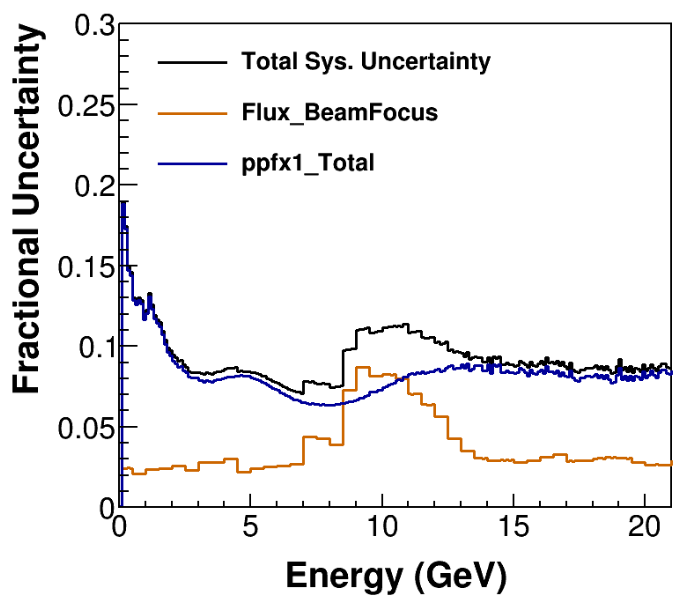
\includegraphics[scale=0.4]{Figures/Chapter6/BeamUncertainties.png}
    \caption{Flux uncertainty breakdown as function of the neutrino energy. The ppfx1\_Total is the total uncertainties produced by the hadron production parameters and the total beam focusing uncertainty. Figure from \cite{BenThesis}.}
    \label{fig:Systematics:FluxUncertainties}
\end{figure} 

The flux uncertainties are one of the biggest components of the total uncertainty in the cross section calculation. For the 1D analysis, the variable most affected by this uncertainty is $P^z_\mu$, this uncertainty is between 8\% and 3\% for all variables. In the 2D analysis, the combination of the more affected variables is $P^T_\mu$ with $P^z_\mu$. The uncertainty is between 6\% and 3\%. In the \textbf{Appendix} \ref{Ap:Systematics1D:Flux} the plots with the systematic uncertainties are reported for 1D and 2D analyzes. 

\subsection{Others}
\label{Cap:ErrorAnalysis:SystematicUnc:Others}

This group of uncertainties includes uncertainties related to the target mass, particle response, and GEANT4 uncertainties. 

The target mass shifts the density of the material, it has an effect on dE/dx reconstruction, particle identification reconstruction, and the calculation of the number of targets in the detector. For these analyses, it only shifts the mass density of the plastic scintilator situated in the tracker region.  

The particle response uncertainties shift the calorimetric energy response of the detector. It is specific for each particle. The sources of the variations effects for different sources such as calibration, Geant4 model, etc. These uncertainties were measured using data from the Miner$\nu$A testbeam detector\cite{TestBeamPion}\cite{TestBeamProton}. The response was measured using a beam of protons, pions, and electrons with a well-known energy. This uncertainty affects the reconstructed recoil energy, which is used to estimate the hadronic energy and other variables such as $W_{exp}$, $Q^2$ and $E_\nu$.

The GEANT4 uncertainties are related to the models that are used to simulate the trajectory inside the detector and the secondary inelastic interactions of the particles in the detector. Initially, these effects are not included in the simulation; therefore, an weight is applied to simulate these effects, reducing or increasing the probability of the secondary inelastic interactions. 

\begin{table}[!htb]
    \centering
    \begin{tabular}{c|p{2in}|c|c|c}
        \hline 
        Parameter & Description  & Shift (1 $\sigma$) & \multicolumn{2}{c}{Effect} \\
         & & & 1D & 2D \\
        \hline  
        GEANT\_Neutron & Shift the probability of secondary interactions for a neutron.  & $\pm10\%$ & $>1\%$ & $>1.3\%$\\ \hline
        GEANT\_Pion & Shift the probability of secondary interactions for a pion. & $\pm10\%$ & $>2.5\%$ & $>2.9\%$ \\ \hline
        GEANT\_Proton & Shift the probability of secondary interactions for a proton. & $\pm10\%$ & $>0.5\%$ & $>4\%$ \\ \hline
        Target\_Mass\_CH & Variation of the plastic scintillator density. & $\pm1.4\%$ & $>1.5\%$ & $>0.002\%$\\ \hline
        response\_em & It shifts the hadronical recoil energy for the production of electrons and photons. & $\pm3\%$ & $>0.25\%$ & $>1.6\%$ \\ \hline
        response\_meson & It shifts the hadronical recoil energy for the production of mesons. & $\pm5\%$ & $>1\%$ & $>2.2\%$\\ \hline
        response\_proton & It shifts the hadronical recoil energy for the production of protons. & $\pm3.5\%$ & $>0.9\%$ & $>4.4\%$\\ \hline
        response\_other & It shifts the hadronical recoil energy for the production of other particles.& $\pm40\%$ & $>1.6\%$ & $>2.7\%$\\ \hline
    \end{tabular}
    \caption{The systematic uncertainty description for the Geant4, detector response and mass detector shifts and their effect in the cross section results are shown. }
    \label{tab:ErrorAnalysis:SystematicUnc:Other}
\end{table}


\pagebreak

\section{Cross Section Systematic Uncertainties}
\label{Cap:ErrorAnalysis:CrossSectionUncertainties}

In this section the results for the 1D and the 2D analysis systematic uncertainties summaries are shown. The breakdown plots for each systematic uncertainty can be found in the \textbf{Appendix} \ref{Ap:Systematics1D}.

\foreach \var in  {enu,mixtpi,mixthetapi_deg,pmu,ptmu,pzmu,thetamu_deg,q2,wexp}{
%\foreach \var in  {enu_true,mixtpi_true,pmu_true,ptmu_true,pzmu_true,thetamu_deg_true,q2_true,wexp_true}{
    \ifthenelse{\equal{\var}{enu}}{
      \renewcommand{\NewVar}{E_\nu}
    }{}
    \ifthenelse{\equal{\var}{mixtpi}}{
      \renewcommand{\NewVar}{T_\pi}
    }{}
    \ifthenelse{\equal{\var}{mixthetapi_deg}}{
      \renewcommand{\NewVar}{\theta_\pi}
    }{}
    \ifthenelse{\equal{\var}{pmu}}{
      \renewcommand{\NewVar}{P_\mu}
    }{}
    \ifthenelse{\equal{\var}{ptmu}}{
      \renewcommand{\NewVar}{P^T_\mu}
    }{}
    \ifthenelse{\equal{\var}{pzmu}}{
      \renewcommand{\NewVar}{P^z_\mu}
    }{}
    \ifthenelse{\equal{\var}{thetamu_deg}}{
      \renewcommand{\NewVar}{\theta_\mu}
    }{}
    \ifthenelse{\equal{\var}{q2}}{
      \renewcommand{\NewVar}{Q^2}
    }{}
    \ifthenelse{\equal{\var}{wexp}}{
      \renewcommand{\NewVar}{W_{exp}}
    }{}
    \begin{figure}
        \centering
        \includegraphics[scale=0.3]{Figures/AppendixB/XsecUnc1D/ErrorSummary_CrossSection_\var_Frac__1Pi_.png}
        \caption{$\NewVar$ 1D Cross Section error summary, including the statistical and systematic uncertainties breakdown per group. Figure by the author.}
        \label{fig:Systematics:1DSystematics\var}
    \end{figure}  
}

\foreach \var in  {ptmu_vs_tpi,tpi_vs_ptmu,ptmu_vs_pzmu,pzmu_vs_ptmu,tpi_vs_pmu,pmu_vs_tpi,thetapi_deg_vs_tpi,tpi_vs_thetapi_deg,enu_vs_tpi,tpi_vs_enu}{


    \ifthenelse{\equal{\var}{pzmu_vs_ptmu}}{
      \renewcommand{\NewVar}{P^z_\mu,P^T\mu}
    }{}
    \ifthenelse{\equal{\var}{tpi_vs_thetapi_deg}}{
      \renewcommand{\NewVar}{T_\pi,\theta_\pi}
    }{}
    \ifthenelse{\equal{\var}{tpi_vs_pmu}}{
      \renewcommand{\NewVar}{T_\pi,P_\mu}
    }{}
    \ifthenelse{\equal{\var}{ptmu_vs_tpi}}{
      \renewcommand{\NewVar}{P^T_\mu, T_\pi}
    }{}
    \ifthenelse{\equal{\var}{ptmu_vs_pzmu}}{
      \renewcommand{\NewVar}{P^T\mu, P^z_\mu}
    }{}
    \ifthenelse{\equal{\var}{thetapi_deg_vs_tpi}}{
      \renewcommand{\NewVar}{\theta_\pi, T_\pi}
    }{}
    \ifthenelse{\equal{\var}{pmu_vs_tpi}}{
      \renewcommand{\NewVar}{P_\mu, T\pi}
    }{}
    \ifthenelse{\equal{\var}{tpi_vs_ptmu}}{
      \renewcommand{\NewVar}{T_\pi,P^T_\mu}
    }{}
    \ifthenelse{\equal{\var}{tpi_vs_enu}}{
      \renewcommand{\NewVar}{T_\pi,E_\nu}
    }{}
    \ifthenelse{\equal{\var}{enu_vs_tpi}}{
      \renewcommand{\NewVar}{E_\nu, T_\pi}
    }{}
    \begin{figure}
        \centering
        \includegraphics[scale=0.3]{Figures/AppendixC/2D_ErrorSummary_CrossSection_\var_.png}
        \caption{$\NewVar$ 2D Cross Section error summary, including the statistical and systematic uncertainties breakdown per group. Figure by the author.}
        \label{fig:Systematics:2DSystematics\var}
    \end{figure}  
}
